%% Developers manual for C++ BOUT code

\documentclass[12pt]{article}
\usepackage[nofoot]{geometry}
\usepackage{graphicx}
\usepackage{fancyhdr}

\usepackage{listings}
\usepackage{color}
\usepackage{textcomp}
\definecolor{listinggray}{gray}{0.9}
\definecolor{lbcolor}{rgb}{0.95,0.95,0.95}
\lstset{
	backgroundcolor=\color{lbcolor},
        language=C++,
	keywordstyle=\bfseries\ttfamily\color[rgb]{0,0,1},
	identifierstyle=\ttfamily,
	commentstyle=\color[rgb]{0.133,0.545,0.133},
	stringstyle=\ttfamily\color[rgb]{0.627,0.126,0.941},
	showstringspaces=false,
	basicstyle=\small,
	numberstyle=\footnotesize,
	numbers=left,
	stepnumber=1,
	numbersep=10pt,
	tabsize=2,
	breaklines=true,
	prebreak = \raisebox{0ex}[0ex][0ex]{\ensuremath{\hookleftarrow}},
	breakatwhitespace=false,
	aboveskip={1.5\baselineskip},
        columns=fixed,
        upquote=true,
        extendedchars=true,
}

%% Modify margins
\addtolength{\oddsidemargin}{-.25in}
\addtolength{\evensidemargin}{-.25in}
\addtolength{\textwidth}{0.5in}
\addtolength{\textheight}{0.25in}
%% SET HEADERS AND FOOTERS

\pagestyle{fancy}
\fancyfoot{}
\renewcommand{\sectionmark}[1]{         % Lower case Section marker style
  \markright{\thesection.\ #1}}
\fancyhead[LE,RO]{\bfseries\thepage}    % Page number (boldface) in left on even
                                        % pages and right on odd pages 
\renewcommand{\headrulewidth}{0.3pt}

\newcommand{\code}[1]{\texttt{#1}}
\newcommand{\file}[1]{\texttt{\bf #1}}

%% commands for boxes with important notes
\newlength{\notewidth}
\addtolength{\notewidth}{\textwidth}
\addtolength{\notewidth}{-3.\parindent}
\newcommand{\note}[1]{
\fbox{
\begin{minipage}{\notewidth}
{\bf NOTE}: #1
\end{minipage}
}}

\newcommand{\pow}{\ensuremath{\wedge} }
\newcommand{\poweq}{\ensuremath{\wedge =} }

\newcommand{\deriv}[2]{\ensuremath{\frac{\partial #1}{\partial #2}}}

\newcommand{\rbtsq}{\ensuremath{\left(RB_\theta\right)^2}}
\newcommand{\sbt}{\ensuremath{\sigma_{B\theta}}}
\newcommand{\apar}{\ensuremath{A_{||}}}
\newcommand{\Bthe}{\ensuremath{B_\theta}}
\newcommand{\Bzeta}{\ensuremath{B_\zeta}}
\newcommand{\hthe}{\ensuremath{h_\theta}}

\begin{document}

\title{BOUT++ Developers' Manual}
\author{B.Dudson, University of York}

\maketitle

\tableofcontents

\section{Introduction}

This is a manual describing the core BOUT++ code, and is intended for anyone who
wants to work on improving BOUT++. It does its best to describe
the details of how BOUT++ works, and assumes that the user is very comfortable
with C++. For a general introduction, and instructions for using BOUT++
see the users' guide. The user's guide assumes only minimal knowledge of C++,
and provides only those details needed to use BOUT++. 

Since BOUT++ is a scientific code, it is constantly changing and (hopefully)
being improved. This provides a moving target for documentation, and means
that describing all the details of how BOUT++ works in one document is probably
impossible. This is particularly true since often our first priority is to
write papers and code - not documentation - and so whatever is documented
is likely to be slightly out of date. A source of up-to-date documentation
of the BOUT++ code is the comments and Doxygen tags: running \code{doxygen}
on the source should produce a set of HTML documentation. See
\file{www.doxygen.org} for more details.

\subsection{Collaborating on BOUT++}

As of June 2009, the BOUT++ distribution is hosted on Github:
(\file{http://github.com/bendudson/BOUT/})
If you're just starting with BOUT++, current developers will want to check
your changes before submitting them to the repository. In this case
you should clone (checkout) the git repository, make any changes and
then submit patches to one of the developers (e.g.
to \texttt{bd512@york.ac.uk}). Fortunately Git makes this process quite easy:
The commands to do this are:

First get a copy of BOUT++
\begin{verbatim}
$ git clone git://github.com/bendudson/BOUT.git
\end{verbatim}
Make changes to the repository, including branching, merging etc. Then create
a patch:
\begin{verbatim}
$ 
\end{verbatim}
and then email the patch file to one of the BOUT++ developers. 

If you are doing a lot of development of BOUT++, it will probably make sense
for you to push changes to the online repository.

\subsection{House rules}

BOUT++ consists of about 31,800 lines of C/C++\footnote{generated using
David A. Wheeler's 'SLOCCount'},
along with 11,600 lines of IDL. Of this, about 21,100 lines is the core
BOUT++ code, and the remainder
a mix of pre- and post-processors, and physics modules. As production codes
go, this is not particularly huge, but it is definitely large enough that
keeping the code `clean' and understandable is necessary. This is vital
if many people are going to work on the code, and also greatly helps code
debugging and verification. There are therefore a few house rules to keep
in mind when modifying the BOUT++ code.

When modifying the core BOUT++ code, please keep in mind that this portion of the code
is intended to be general (i.e. independent of any particular physical system of equations),
and to be used by a wide range of users. Making code clear is also more important
in this section than the physics model since the number of developers is potentially
much greater. 

Here are some rules for editing the core BOUT++ code:
\begin{itemize}
\item {\bf NO FORTRAN}. EVER. Though it may be tempting for scientific programmers to use
a little FORTRAN now and then, please please don't put any into BOUT++. 
Use of FORTRAN, particularly when mixed with C/C++, is the cause of many problems in
porting and modifying codes. 
\item If a feature is needed to study a particular system, only include it in the
core code if it is more generally applicable, or cannot be put into the physics module.
\end{itemize}

\section{Code layout}

BOUT++ is organised into classes and groups of functions which operate on them: 
It's not purely object-oriented, but takes advantage of many of C++'s object-oriented features. 

Figure~\ref{fig:layout1} shows the most important parts of BOUT++ and how they fit together.
\begin{figure}[htbp!]
\centering
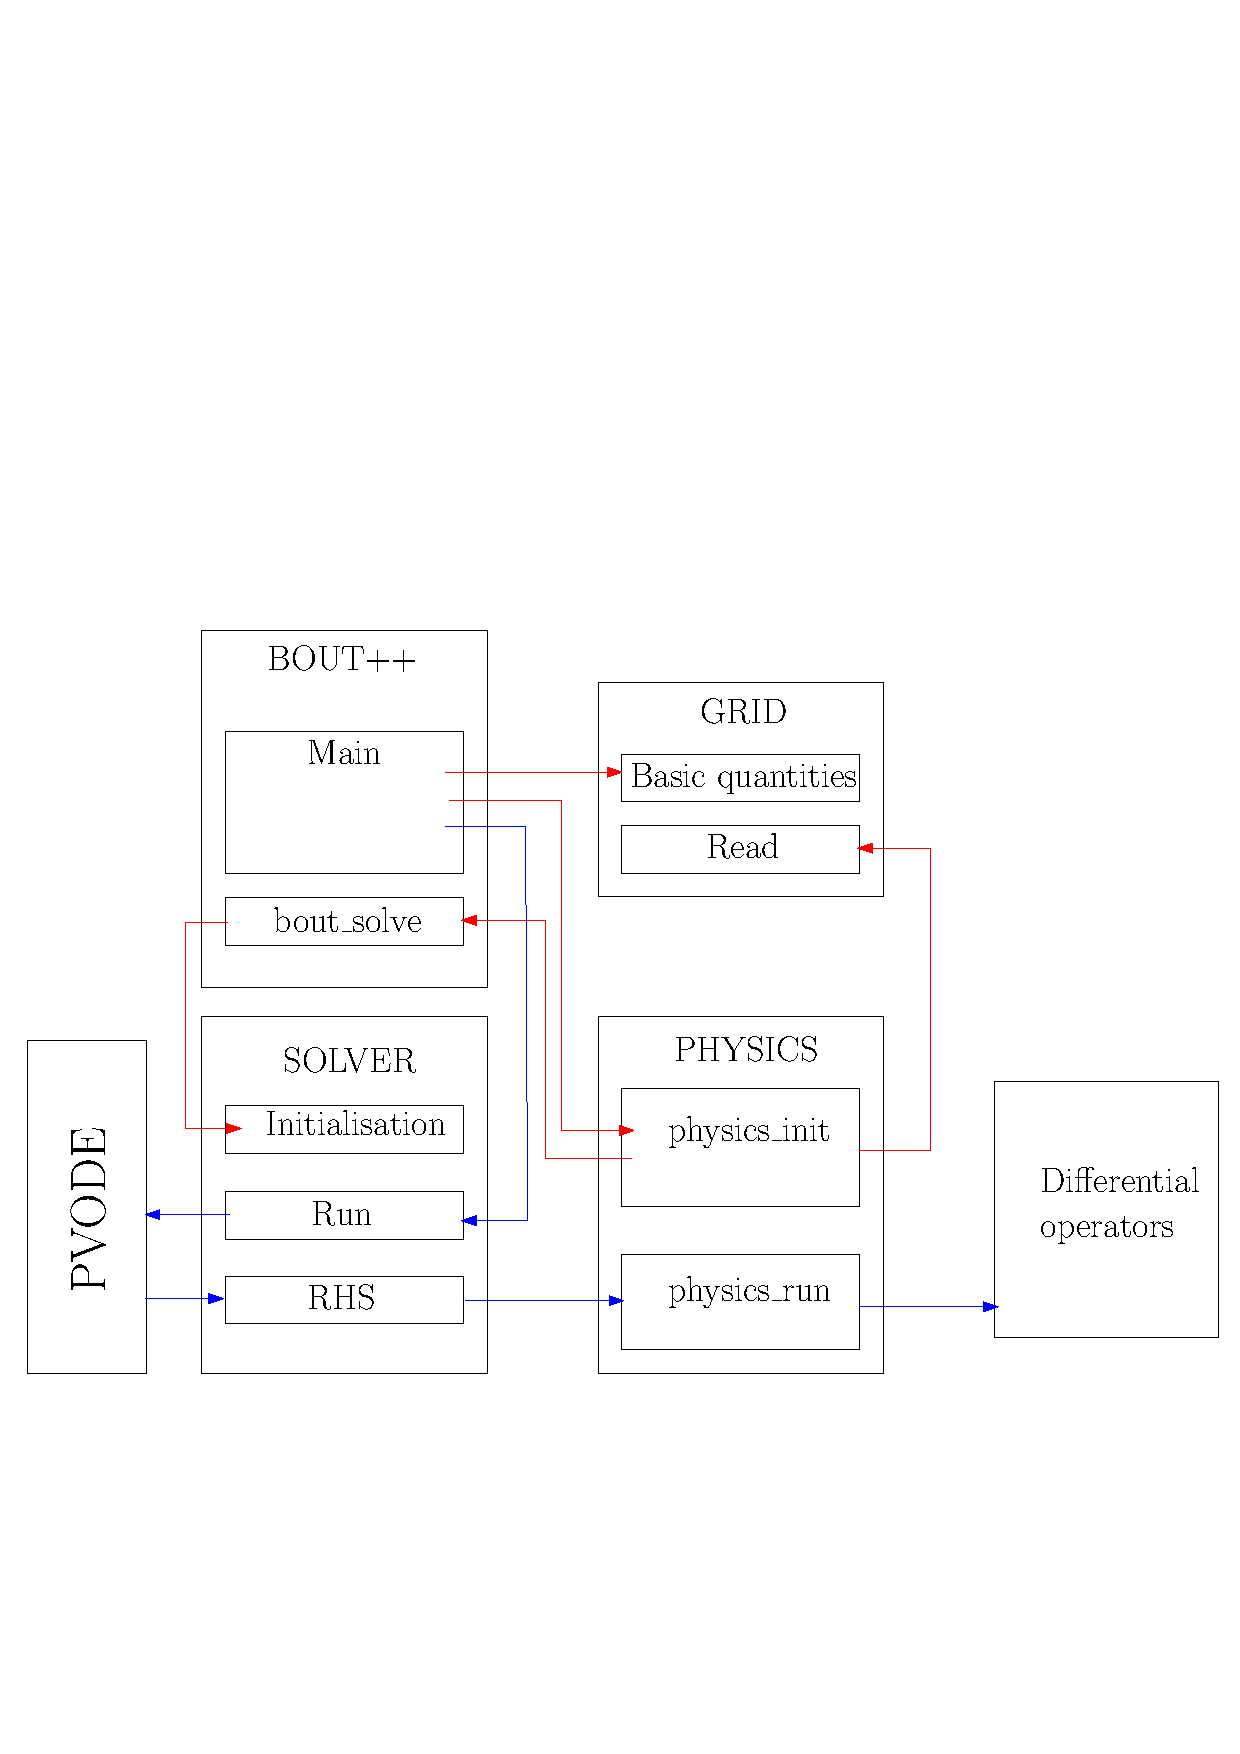
\includegraphics[width=0.7\paperwidth, keepaspectratio]{figs/layout1.pdf}
\caption{Overview of BOUT++ control flow during initialisation (red), and running (blue)}
\label{fig:layout1}
\end{figure}
The initialisation process is shown in red: basic information is first read from the grid
file (e.g. size of the grid, topology etc.), then the user-supplied initialisation
code is called. This code can read other variables from the grid, and makes at least
one call
to \code{bout\_solve} to specify a variable to be evolved. The main thing \code{bout\_solve}
does is to add these variables to the solver. 

The process of running a timestep is shown in blue in figure~\ref{fig:layout1}:
The main loop calls the solver, which in turn calls PVODE. To evolve the system
PVODE makes calls to the RHS function inside solver. This moves data between PVODE
and BOUT++, and calls the user-supplied \code{physics\_run} code to calculate
time-derivatives. Much of the work calculating time-derivatives involves differential
operators.

Calculation of the RHS function \code{physics\_run}, and handling of data
in BOUT++ involves many different components. Figure~\ref{fig:layout2}
shows (most) of the classes and functions involved, and the relationships
between them. Some thought was put into how this should be organised, but
it has also changed over time, so some parts could be cleaner.
\begin{figure}[htbp!]
\centering
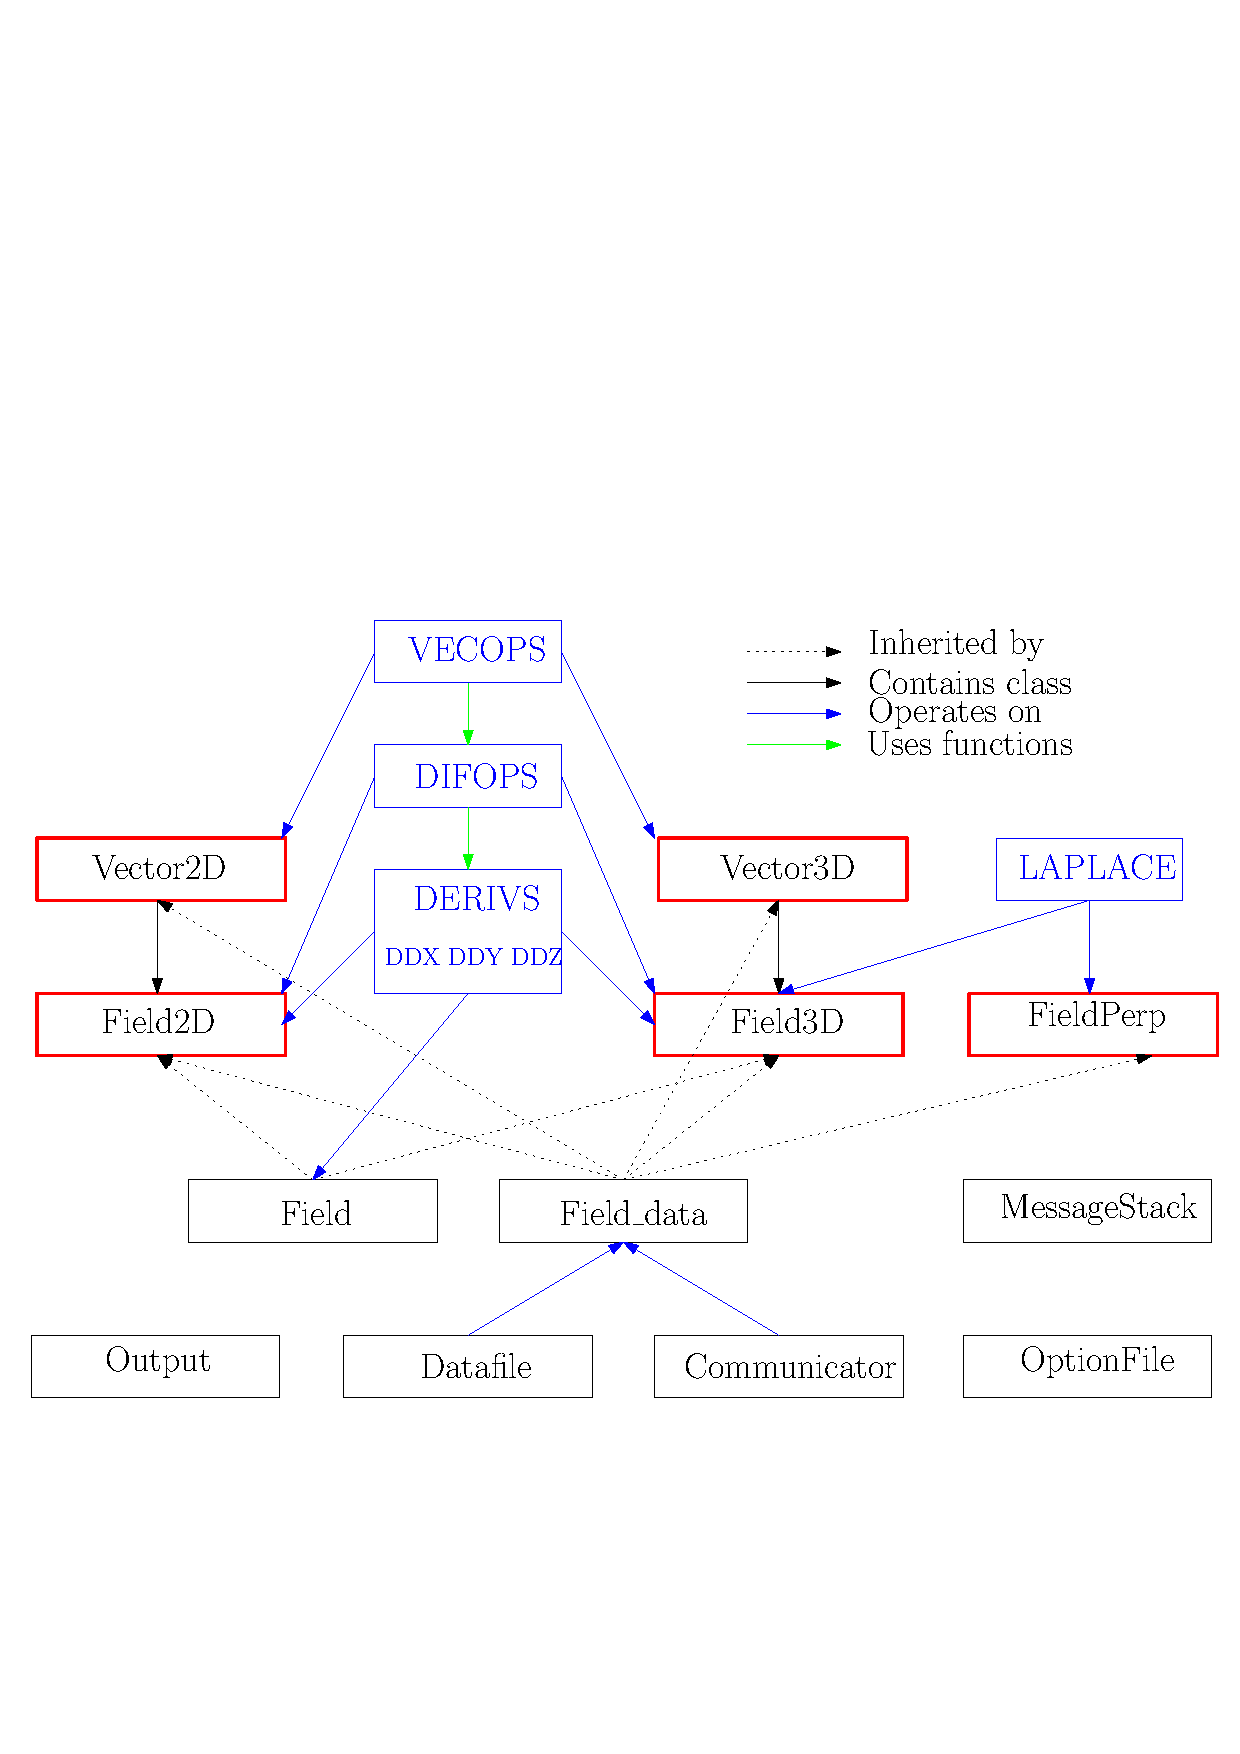
\includegraphics[width=0.6\paperwidth, keepaspectratio]{figs/layout2.pdf}
\caption{Relationship between important classes and functions used in calculating the RHS function}
\label{fig:layout2}
\end{figure}

\subsection{Data types}

The classes outlines in red in figure~\ref{fig:layout2} are data types 
currently implemented in BOUT++. 

\subsubsection{\code{Field}}

The two main types are \code{Field2D}, and \code{Field3D}. Their main functions
are to provide an easy way to manipulate data; they take care of all memory management,
and most looping over grid-points in algebraic expressions. The 2D field implementation
is relatively simple, but more optimisations are used in the 3D field implementation
because they are much larger (factor of $\sim 100$).

\subsubsection{\code{Vector}}

Vector classes build on the field classes, just using a field to represent
each component. 

\subsubsection{\code{dcomplex}}

Several parts of the BOUT++ code involve FFTs and are therefore much easier to
write using complex numbers. Unfortunately, the C++ complex library also tries
to define a \code{real} type, which is already defined by PVODE. Several
work-arounds were tried, some of which worked on some systems, but
it was easier in the end to just implement a new class \code{dcomplex} to
handle complex numbers.

\subsection{Memory management}

This code has been thoroughly tested/debugged, and should only be altered
with great care, since just about every other part of BOUT++ depends on this code
working correctly. Two optimisations used in the data objects to speed up code execution
are memory recycling, which eliminates allocation and freeing of memory; and copy-on-change,
which minimises unnecessary copying of data.

Both of these optimisations are done ``behind the scenes'', hidden from the remainder
of the code, and are illustrated in figure~\ref{fig:memory}:
\begin{figure}[htb!]
\centering
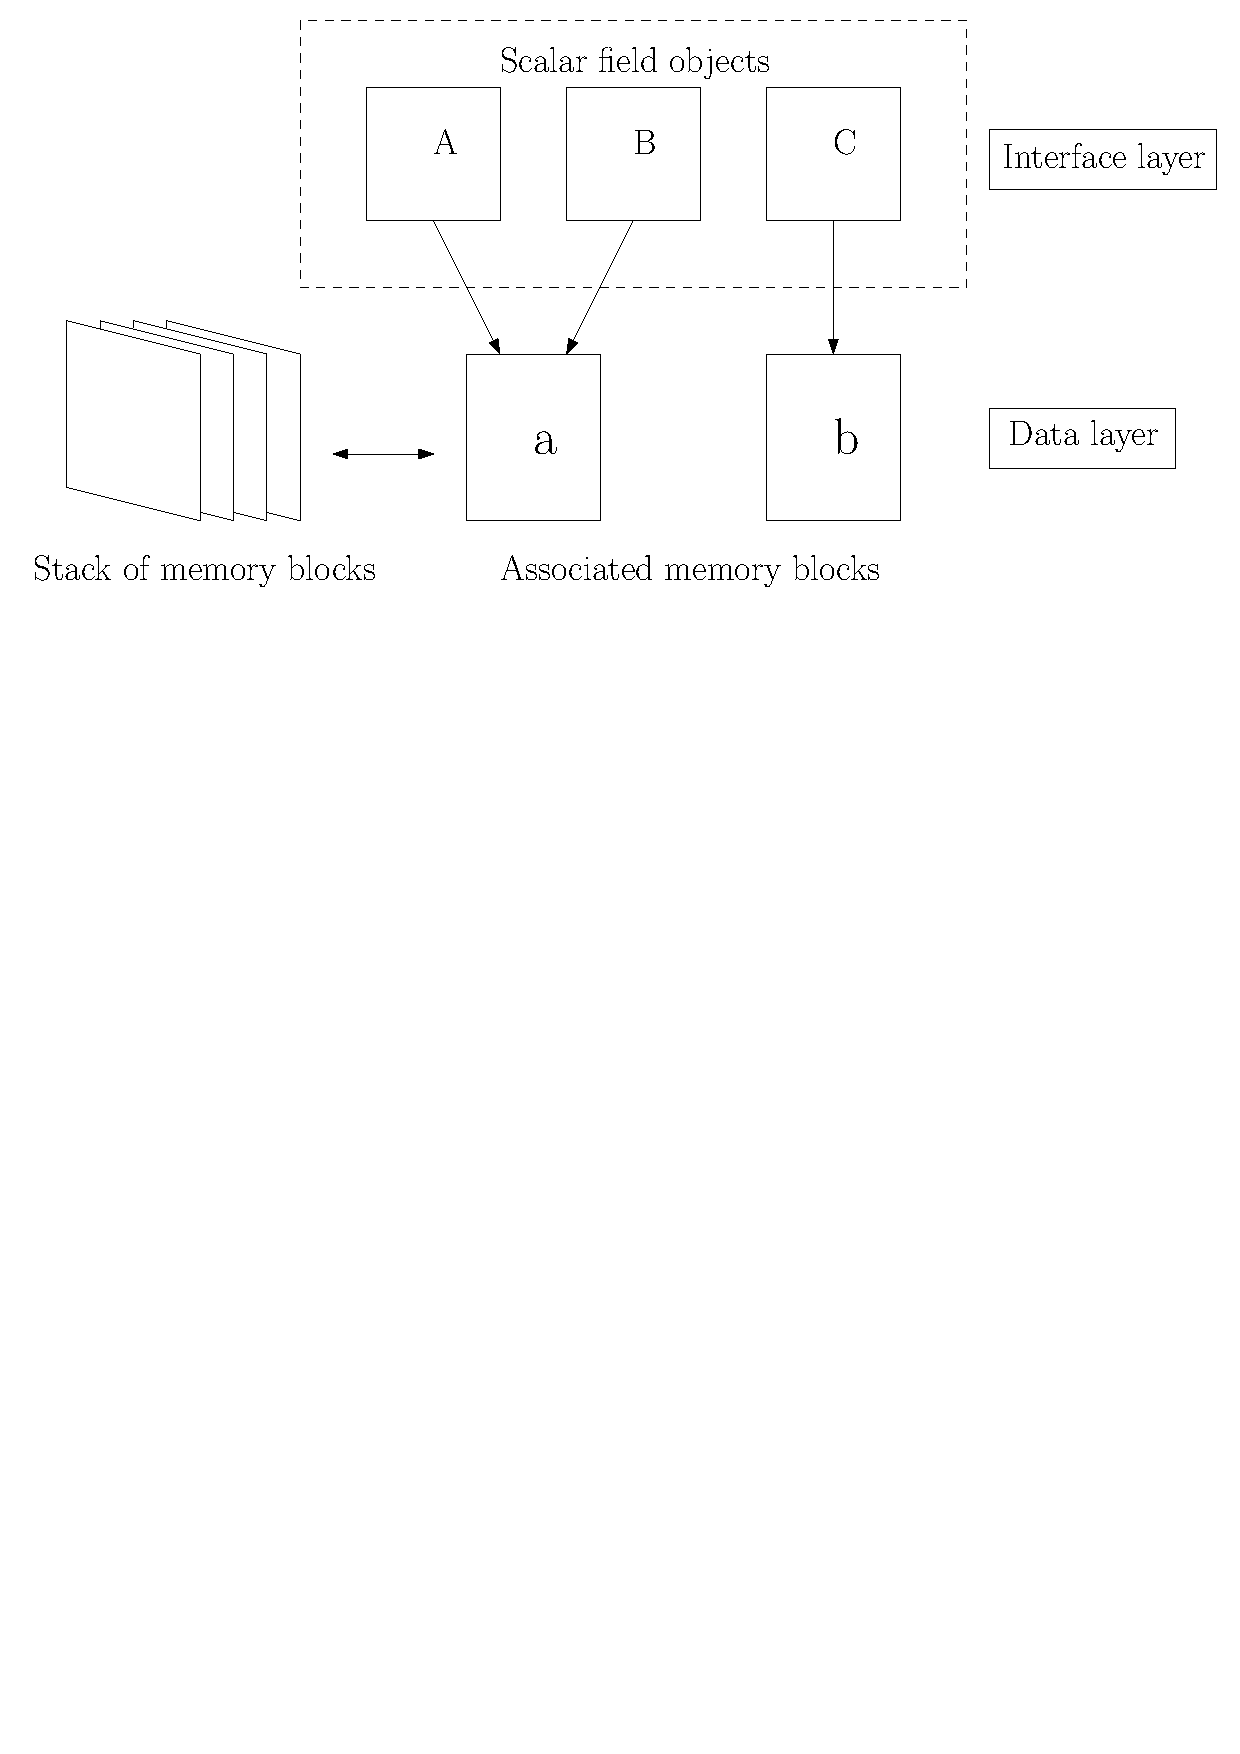
\includegraphics[scale=0.75]{figs/memory.pdf}
\caption{Memory handling in BOUT++. Memory allocation and freeing is eliminated by recycling memory blocks, and assignments without changes (\code{A = B}) do not result in copying data, only pointers to the data. Both these optimisations are handled internally, and are invisible to the programmer.}
\label{fig:memory}
\end{figure}
The objects (A,B,C) accessed by the user in operations
discussed in the previous section act as an interface to underlying data (a,b). 
Memory recycling can be used because all the scalar fields are the same size (and vector fields are
implemented as a set of 3 scalar fields). Each class implements a global stack of available
memory blocks. When an object is assigned a value, it attempts to grab one of these memory blocks,
and if none are available then a new block is allocated. 
When an object is destroyed, its memory block is not freed, but is put onto the
stack. Since the evaluation of the time-derivatives involves the same set of operations each time, this system
means that memory is only allocated the first time the time-derivatives are calculated, after which the same 
memory blocks are re-used. This eliminates the often slow system calls needed to allocate and free memory,
replacing them with fast pointer manipulation. 

Copy-on-change (reference counting) further reduces memory useage and unnecessary copying of data. 
When one field is set equal to another (e.g. \code{Field3D A = B} in figure~\ref{fig:memory}), no 
data is copied, only the reference to the underlying data (in this case both A and B point to data block a). 
Only when one of these objects is modified is a second memory block used to store the different value. 
This is particularly useful when returning objects from a routine. Usually this would
involve copying data from one object to another, and then destroying the original copy. Using
reference counting this copying is eliminated.

\section{Derivatives}

This is probably the part of the code most people will want to alter. The main
task of this module is to map functions on fields like \code{DDX} to direction-independent
differential methods on stencils such as $4^{th}$-order central differencing. This mapping depends on global settings in \file{BOUT.inp}
and is illustrated in figure~\ref{fig:diffOverview}.
\begin{figure}[htb!]
\centering
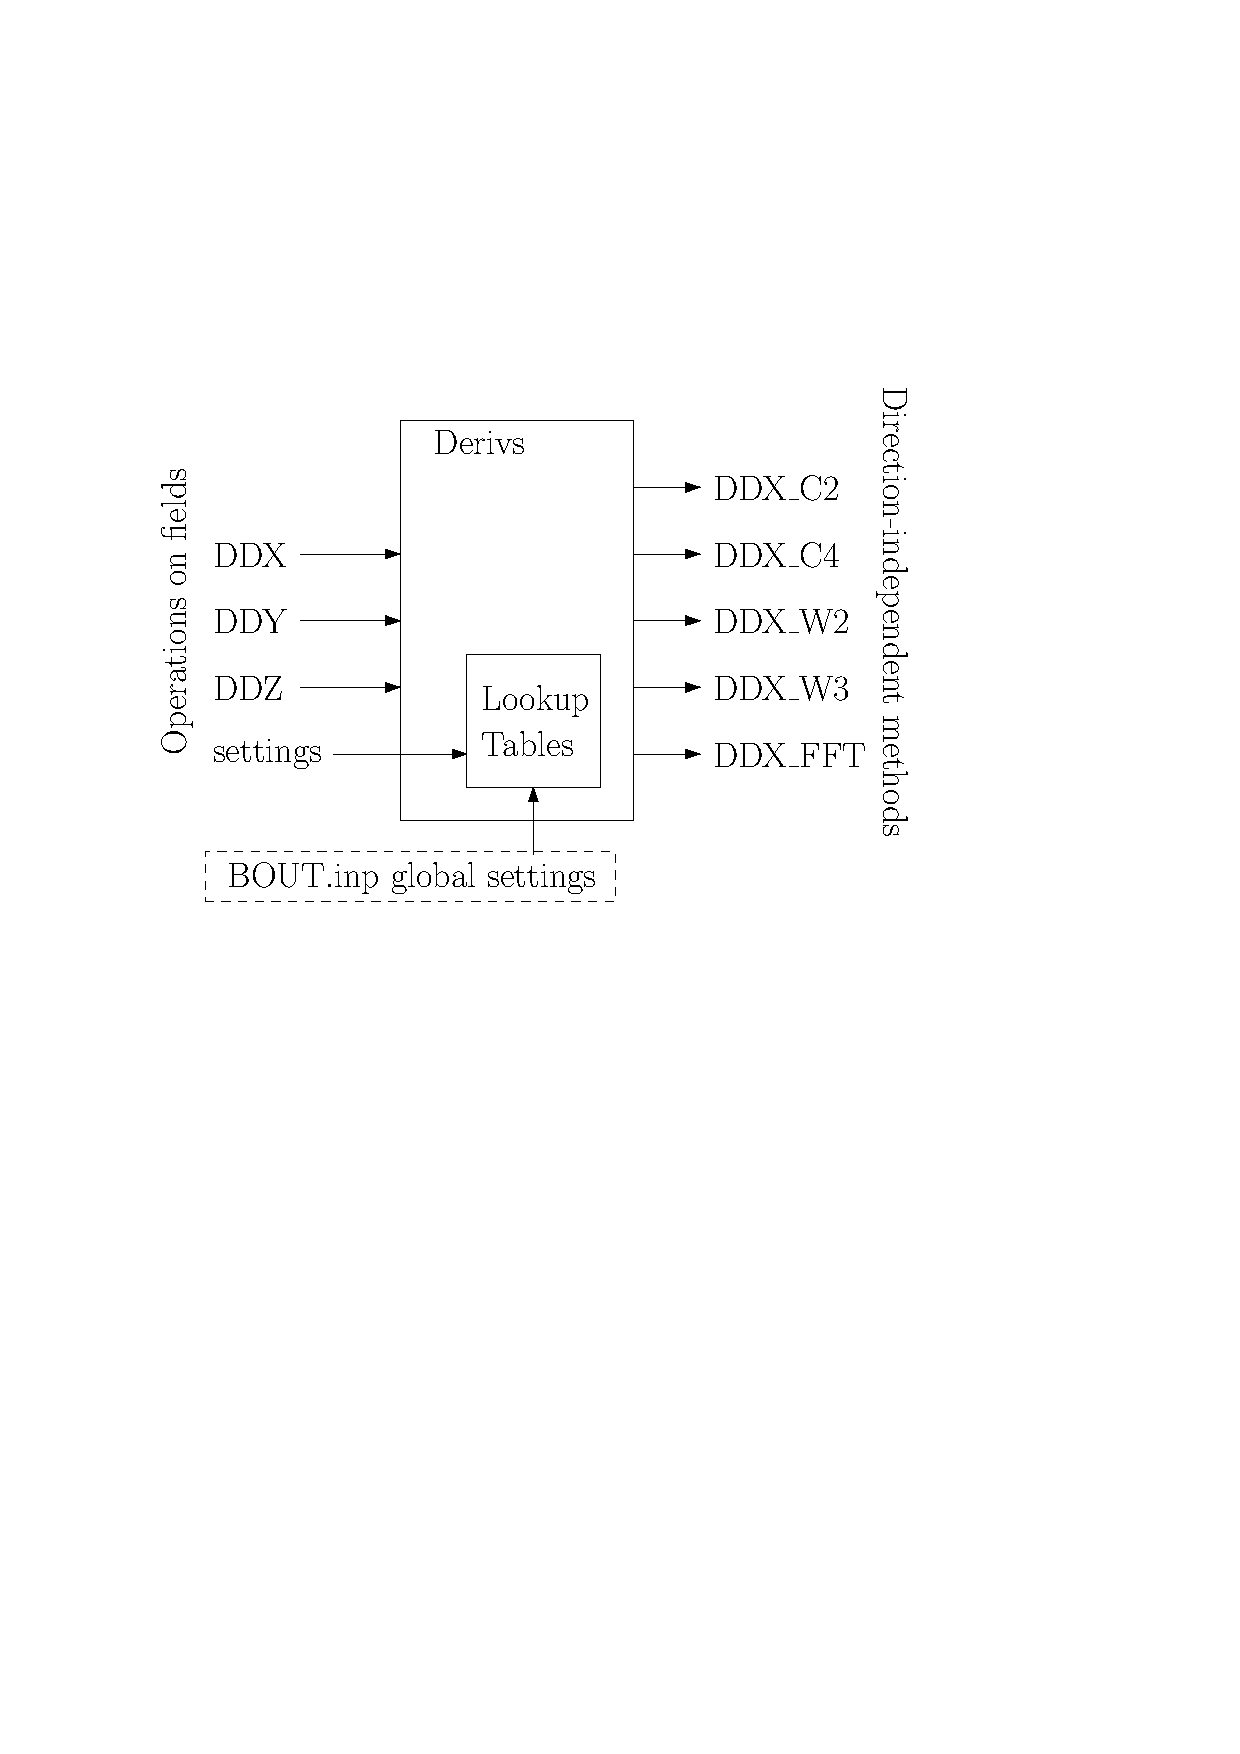
\includegraphics[scale=0.75]{figs/diffOverview.pdf}
\caption{Overview of \code{derivs} module, mapping derivative functions on fields to direction-independent differential methods}
\label{fig:diffOverview}
\end{figure}

The differencing methods themselves are independent on direction, and operate on \code{stencil}
objects. This class is in \file{stencils.h}
\begin{lstlisting}
class stencil {
  public:
    int jx, jy, jz;  // Central location
    real c, p, m, pp, mm; // stencil 2 each side of the centre
    Overloaded operators
      =,+,-,*,/
    Functions
      min, max, abs
};
\end{lstlisting}
The main purpose of this class is to store a 5-element stencil. To simplify some code
this class also has a bunch of overloaded operators on reals and other stencil objects. 
There are also some functions to calculate things like absolute, minimum, and maximum
values.

\subsection{Lookup tables}

Originally, BOUT++ used a load of \code{case} statements to determine
which differencing method to use. 

\begin{figure}[htb!]
\centering
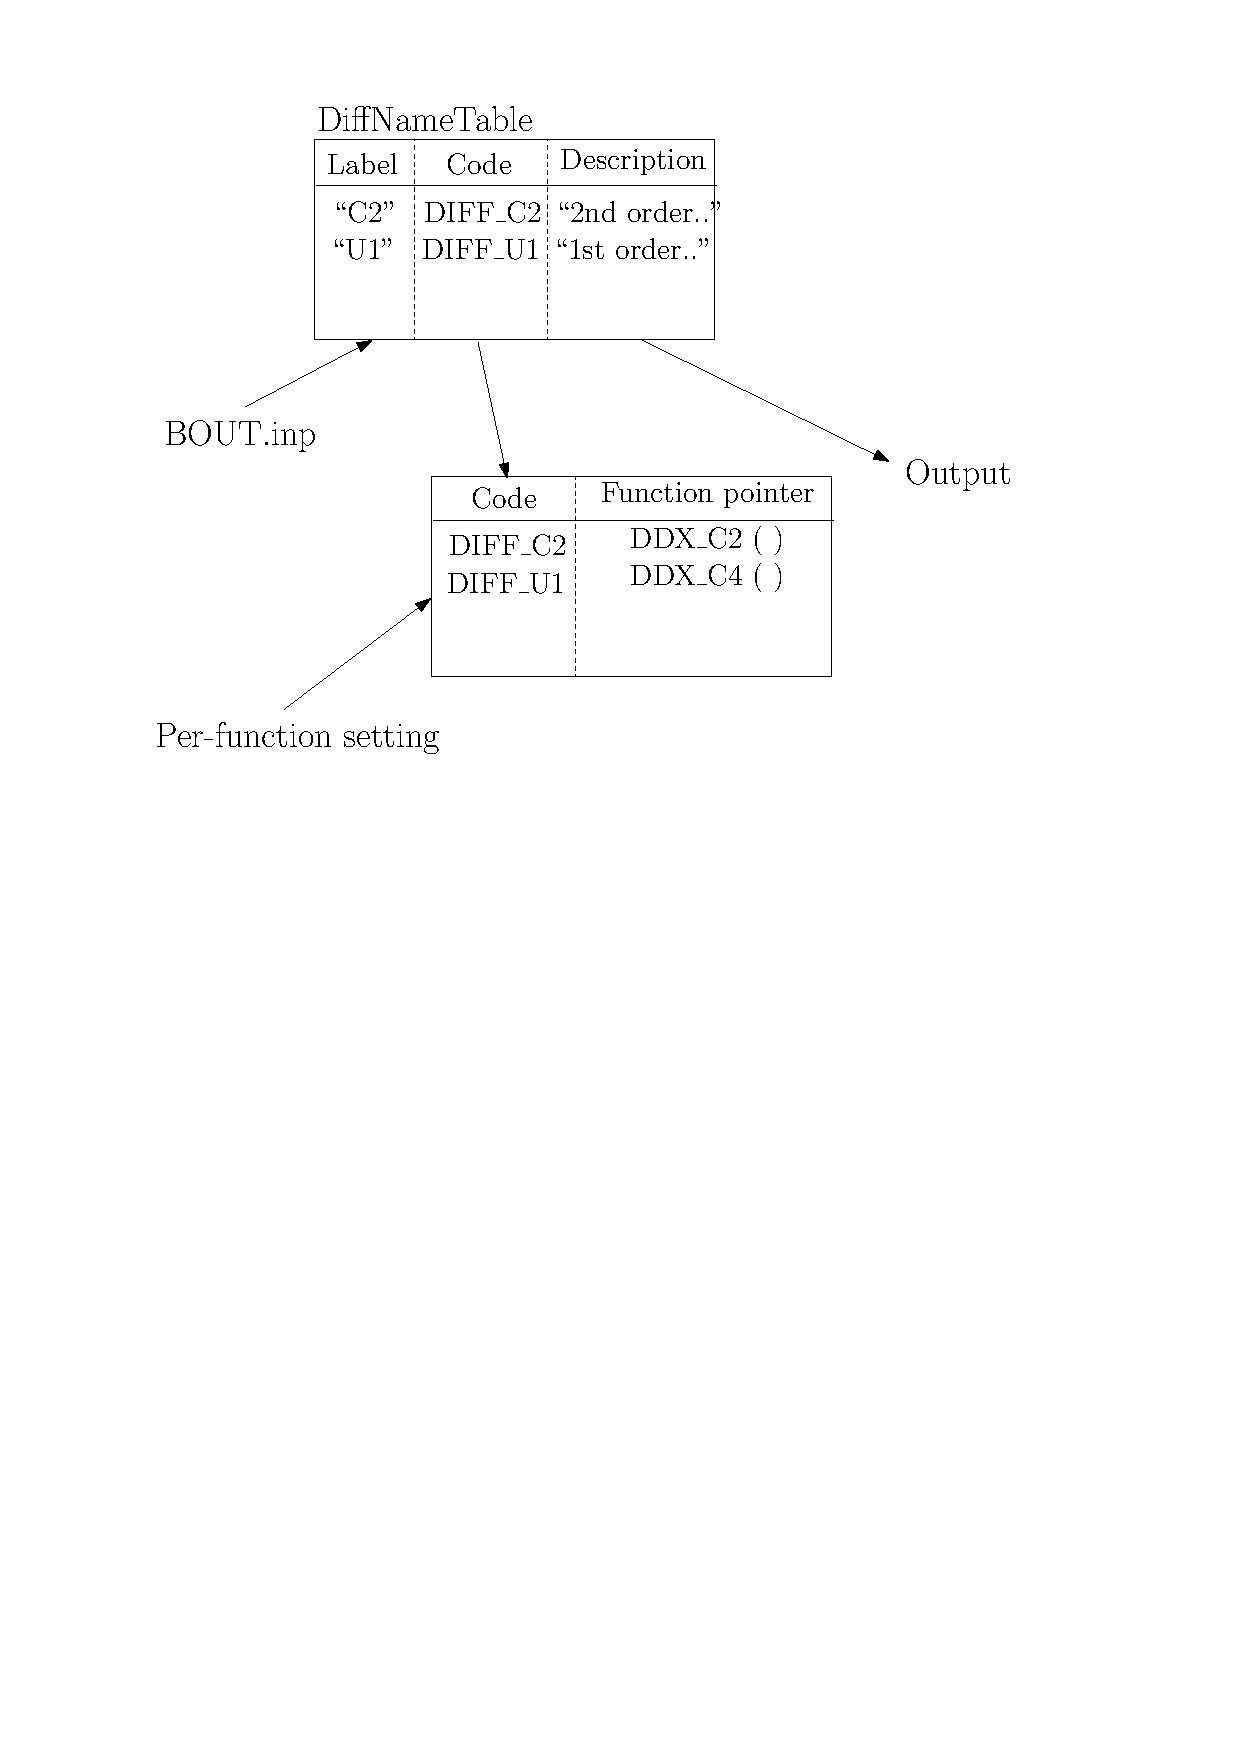
\includegraphics[scale=0.75]{figs/diffLookup.pdf}
\caption{Lookup tables for mapping between differential method labels, codes, descriptions and function pointers}
\label{fig:diffLookup}
\end{figure}

\subsection{Staggered grids}

\note{This feature is currently very experimental, and doesn't appear to work as it should}

By default, all quantities in BOUT++ are defined at cell centre, and
all derivative methods map cell-centred quantities to cell centres.
Switching on staggered grid support in BOUT.inp:
\begin{verbatim}
StaggerGrids = true
\end{verbatim}
allows quantities to be defined on cell boundaries. Functions such as \code{DDX} now have to handle
all possible combinations of input and output locations, in addition to the possible
derivative methods. 

Several things are not currently implemented, which probably should be:
\begin{itemize}
\item Only 3D fields currently have a cell location attribute. The location (cell centre etc) of 2D fields is ignored at the moment. The rationale for this is that 2D fields are assumed to be slowly-varying equilibrium quantities for which it won't matter so much. Still, needs to be improved in future
\item Twist-shift and X shifting still treat all quantities as cell-centred.
\item No boundary condition functions yet account for cell location. 
\end{itemize}

Currently, BOUT++ does not support values at cell corners; values can
only be defined at cell centre, or at the lower X,Y, or Z boundaries. 
This is 

Once staggered grids are enabled, two types of stencil are needed: those
which map between the same cell location (e.g. cell-centred values to cell-centred values), and those which map to different locations (e.g. cell-centred to lower X).

\begin{figure}[htb!]
\centering
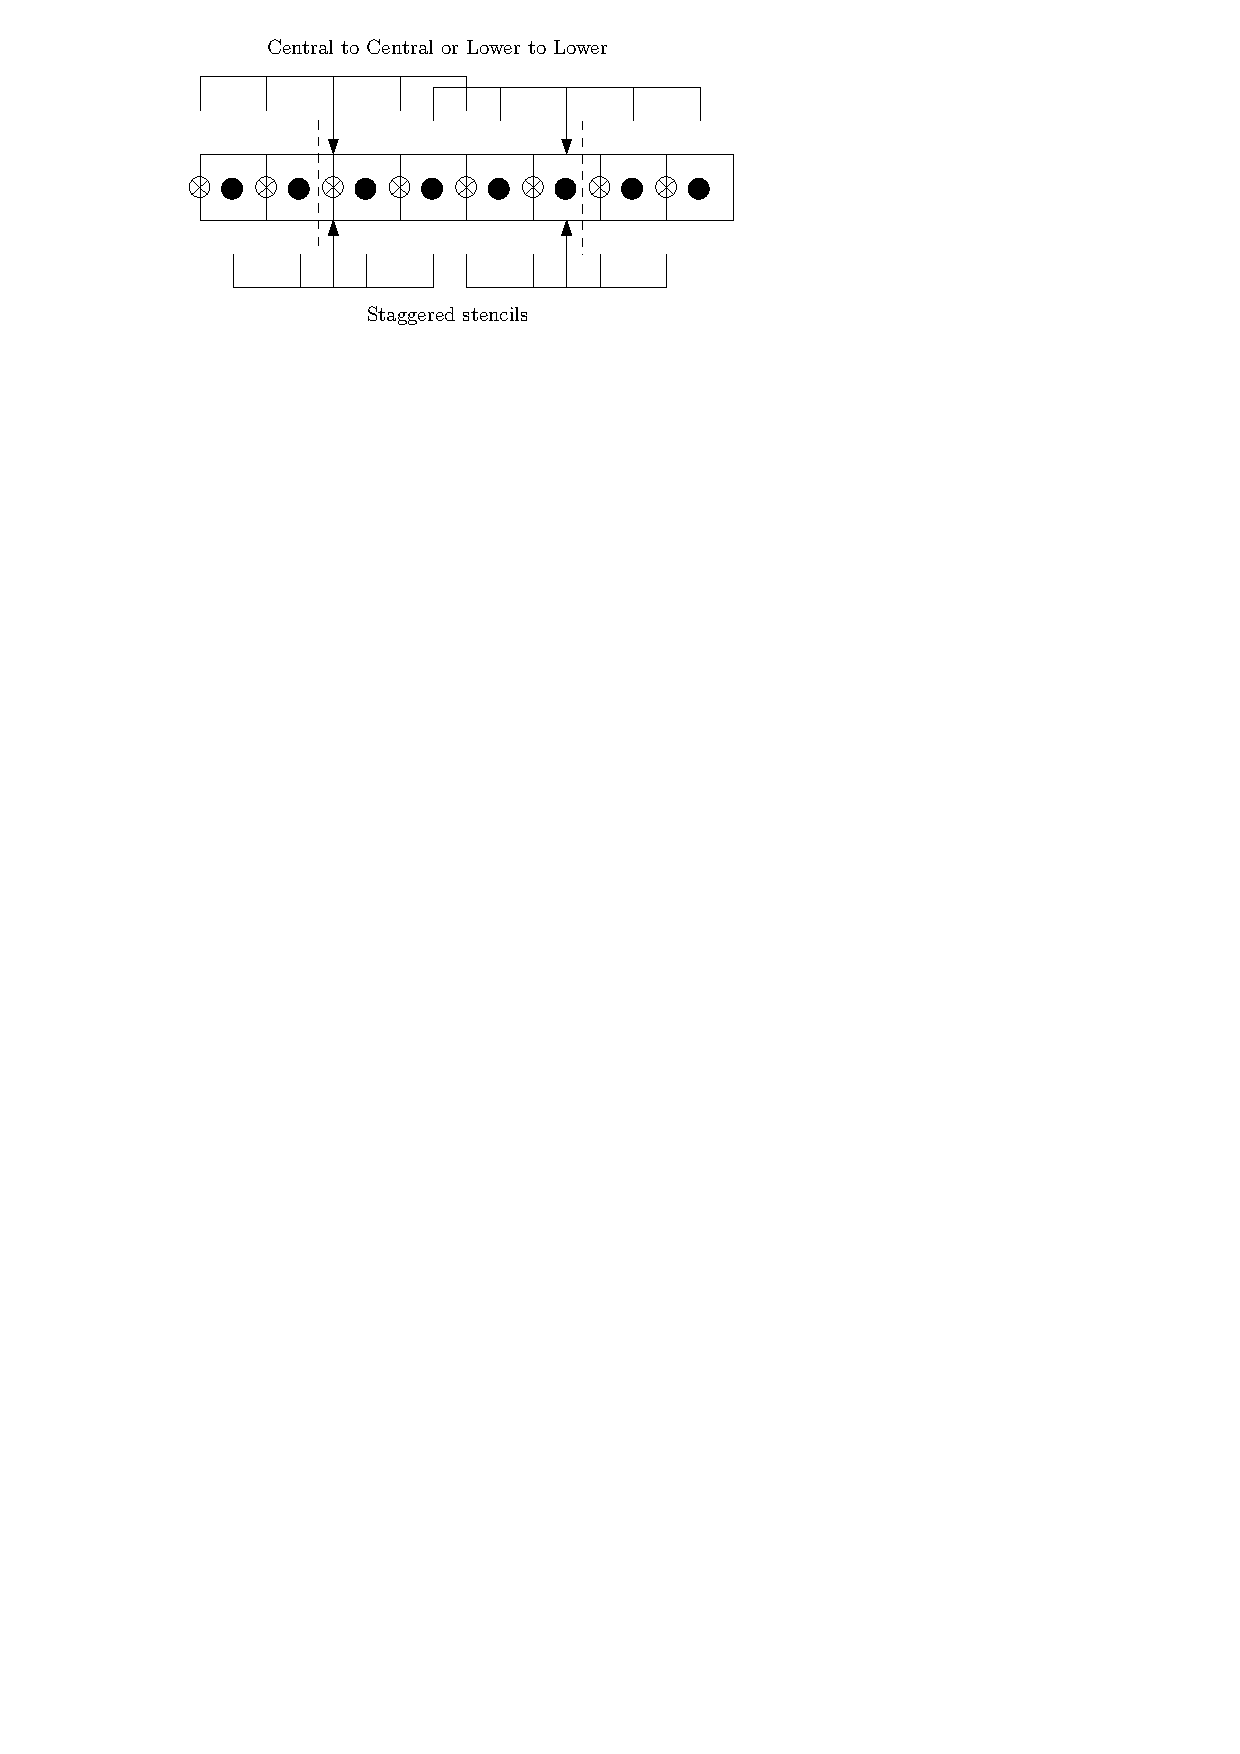
\includegraphics[scale=0.9]{figs/diffStencils.pdf}
\caption{Stencils with cell-centred (solid) and lower shifted values (open). Processor boundaries
marked by vertical dashed line}
\label{fig:diffStencils}
\end{figure}

Central differencing using 4-point stencil:
\begin{eqnarray*}
y &=& \left(9y_{-1/2} + 9y_{1/2} - y_{-3/2} - y_{3/2}\right) / 16 \\
\deriv{y}{x} &=& \left( 27y_{1/2} - 27y_{-1/2} - y_{3/2} + y_{-3/2}\right) / 24\Delta x \\
\frac{\partial^2 y}{\partial x^2} &=& \left(y_{3/2} + y_{-3/2} - y_{1/2} - y_{-1/2}\right) / 2\Delta x^2
\end{eqnarray*}

\note{What should the default cell location of a derivative be? Currently the default is to remain the same as without staggered grids. Setting \code{StaggerGrids = true} by itself has no effect - derivative output locations have to be explicitly set.}

\begin{table}[htbp!]
\caption{DDX actions depending on input and output locations. Uses first match.}
\label{tab:ddxloc}
\centering
\begin{tabular}[c]{c c | l}
\hline
Input & Output & Actions \\
\hline
\multicolumn{2}{c}{Same locations} & Central stencil \\
CENTRE & XLOW & Lower staggered stencil \\
XLOW & CENTRE & Upper staggered stencil \\
XLOW & Any & Staggered stencil to CENTRE, then interpolate \\
CENTRE & Any & Central stencil, then interpolate \\
Any & Any & Interpolate to centre, use central stencil, then interpolate \\
\hline
\end{tabular}
\end{table}

\section{Laplacian inversion}

\note{This part of the code needs some algorithm improvement (better parallel tridiagonal solver).}

Several different algorithms are implemented for Laplacian inversion, and
they differ between serial and parallel versions.
Serial inversion can currently either be done using a tridiagonal solver
(Thomas algorithm), or a band-solver (allowing $4^{th}$-order differencing).

\subsection{Thomas algorithm (serial)}

\subsection{Band solver (serial)}

This is band-solver which performs a $4^{th}$-order inversion. Currently this
is only available when \code{NXPE=1}; when more than one processor is used in $x$,
the Laplacian algorithm currently reverts to $3^{rd}$-order.

\subsection{Thomas algorithm (parallel)}

The current parallel code is a simple parallelisation of the Thomas algorithm
(so only 2nd order). The operations performed are the same as for the
serial code (useful for testing), but this means it is very inefficient.
Figure~\ref{fig:par_laplace} shows the useage of 4 processors inverting a set of 3 poloidal slices
(i.e. MYSUB=3)
\begin{figure}[htbp!]
\centering
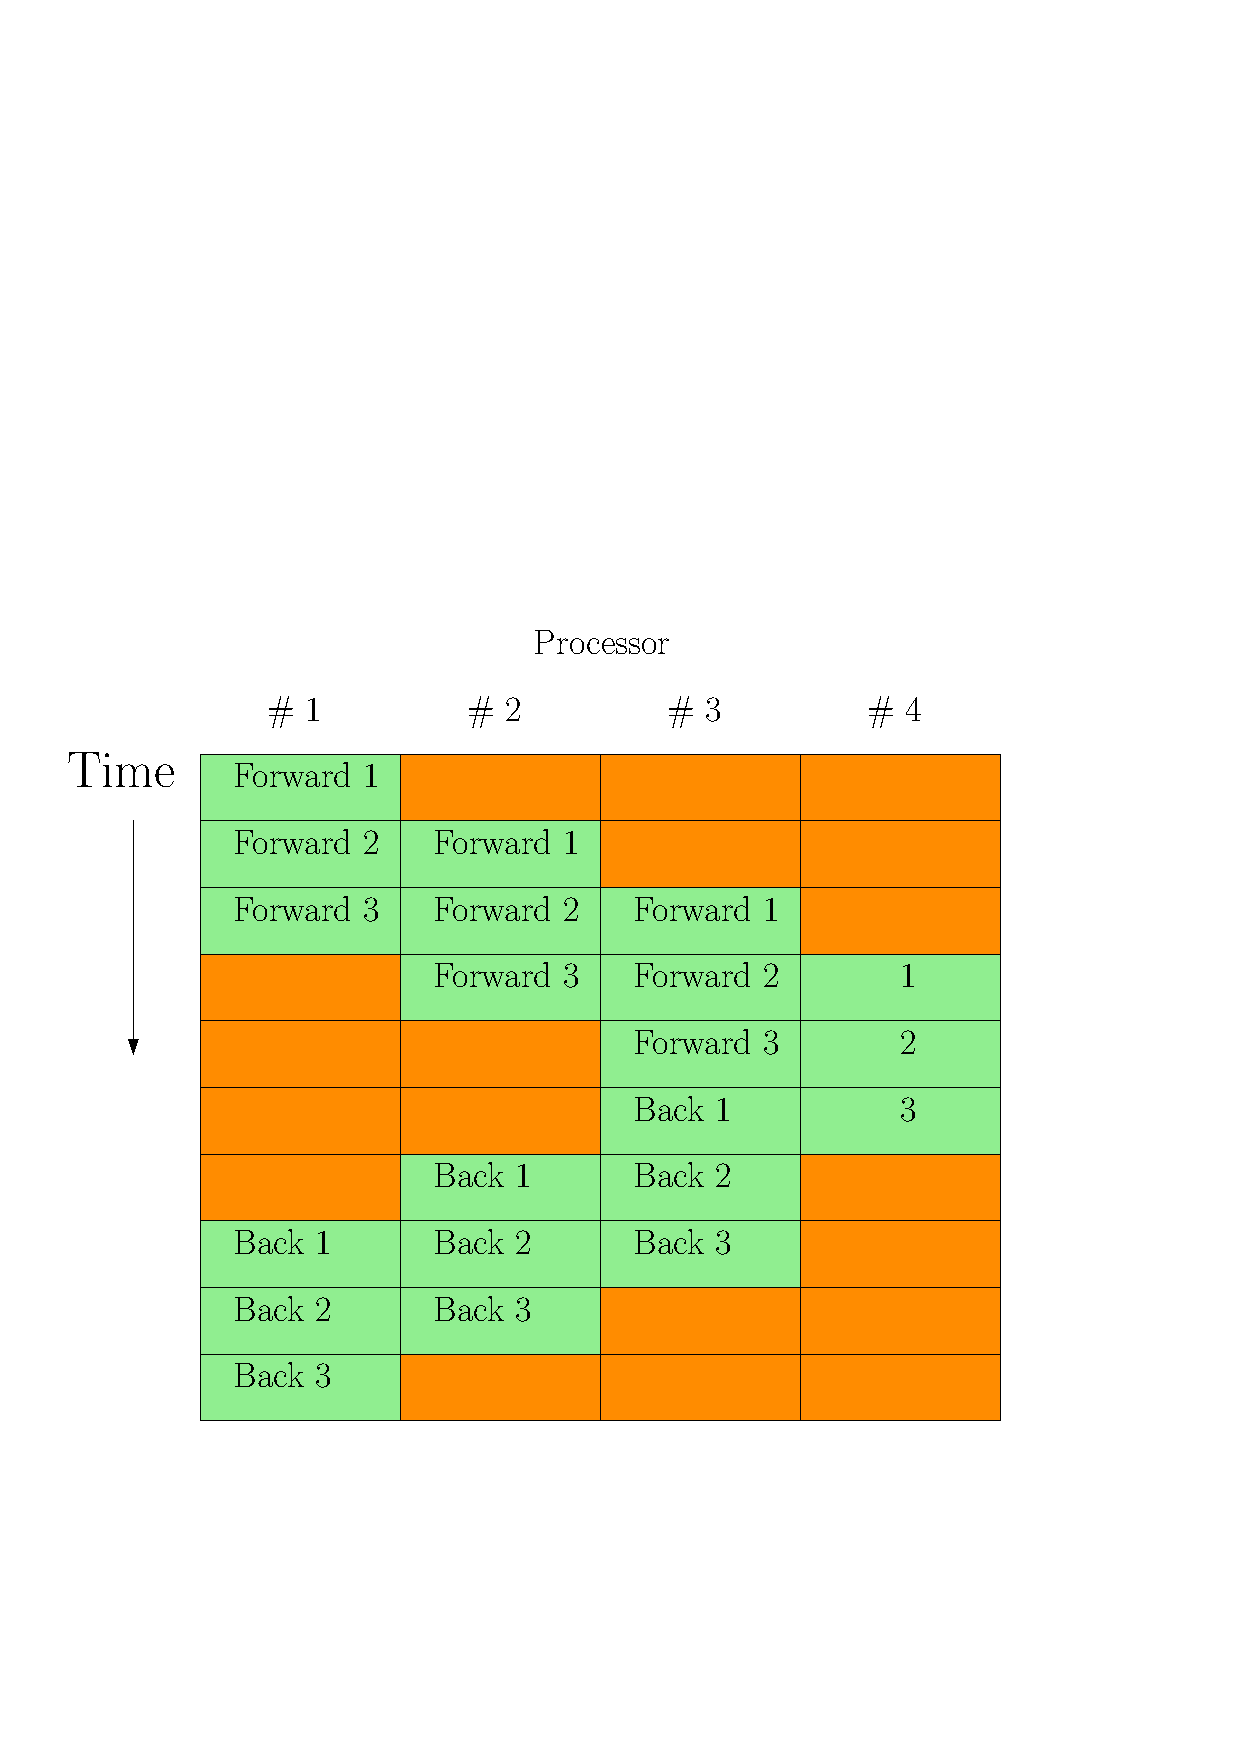
\includegraphics[width=0.5\paperwidth, keepaspectratio]{figs/par_laplace.pdf}
\caption{Parallel Laplacian inversion with MYSUB=3 on 4 processors. Red periods are where a processor is idle - in this case about 40\% of the time}
\label{fig:par_laplace}
\end{figure}

\subsection{PDD algorithm (parallel)}

This is the Parallel Diagonally Dominant (PDD) algorithm. It's very fast, but
achieves this by neglecting some cross-processor terms. For ELM simulations, it has
been found that these terms are important, so this method is not usually used. 

\section{Mesh}

The mesh is used in pretty much all parts of the code, and deals with 
things like the geometry of the mesh (metric tensors etc.), and how the
mesh is divided between processors (communications). The Mesh class
(\file{mesh/mesh.h}) defines an interface, whilst currently BoutMesh
(\file{mesh/boutmesh.h}) is the only implementation of this interface.

\subsection{Loading a mesh}

To load in a mesh from a file or other source, there are the commands:
\begin{lstlisting}
int add_source(GridDataSource);   // Add a data source
int load();                       // Load from added data sources
int load(GridDataSource);         // Load from specified data source
\end{lstlisting}
all of which return an error code (0 if successful). 
\code{add\_source} is used to add a set of input data sources which
inherit from \code{GridDataSource}. \code{load()} loads the mesh
from these sources, querying each data source in turn for the required
variables (in the order in which they were added). \code{load(GridDataSource)}
loads the mesh from only the supplied data source.

In \file{bout++.cpp}, this is used to initialise the mesh:
\begin{lstlisting}
mesh->add_source(new GridFile(data_format(grid_name), grid_name));
if(mesh->load()) {
  output << "Failed to read grid. Aborting\n";
  return 1;
}
\end{lstlisting}
which creates a \code{GridFile} object based on the data format of 
the grid file name, then adds that as a source of data for Mesh.

\subsubsection{Implementation: BoutMesh}



\subsection{Getting data}

The \code{load()} code above needs to read data for the mesh, and physics
codes usually need to read their initial profiles during initialisation.
To do this, Mesh provides an overloaded function \code{get}:
\begin{lstlisting}
int get(var, const char *name); // Request data from mesh file
\end{lstlisting}
where \code{var} can be just about any BOUT++ datatype (\code{Field2D},
\code{Vector3D} etc.). 

\subsubsection{Implementation: BoutMesh}

For integers and reals, the implementation is fairly trivial. Uses
the Mesh protected functions to find a data source and read data from it.
\begin{lstlisting}
GridDataSource* s = find_source(name);  // Find a source of data
s->open(name);                          // Open the source
bool success = s->fetch(&ival, name);   // Get the data
s->close();                             // Close the source
\end{lstlisting}

To read 2D and 3D fields, the branch-cuts need to be taken into account.

\subsection{Communications}

The most common type of communication is to just exchange all
guard cells with neighboring processors. Mesh provides the following
commands for doing this:
\begin{lstlisting}
int communicate(FieldData, ...); // Communicate one or more fields
int communicate(FieldGroup);     // Communicate a group of fields
int communicate(FieldData);      // Returns error code
comm_handle send(FieldGroup);    // Send data
int wait(comm_handle);           // Receive data
\end{lstlisting}
\code{communicate(FieldData)} can (currently) be used to communicate
up to 4 variables together, and makes the code quite clear. For example in
\file{examples/DriftInstability/2fluid.cpp} around line 360:
\begin{lstlisting}
// Need to communicate jpar
mesh->communicate(jpar);
\end{lstlisting}
Since this uses the \code{FieldData} interface like Datafile, this can
be used to communicate all BOUT++ field data types. The limit of 4 is
because the C-style \code{varargs} system doesn't work with ``non POD''
variables, i.e. classes. To communicate a larger number of variables,
create a \code{FieldGroup} object to group fields together, then communicate
them all together:
\begin{lstlisting}
FieldGroup comgrp;  // Group of variables for communication
Field3D P;
Vector3D V;

comgrp.add(P); // Add the variables
comgrp.add(V); // Usually done in physics_init

mesh->communicate(comgrp); // Communicate in physics_run
\end{lstlisting}

If you want to overlap communications with calculations then
use the \code{send} and \code{wait} functions instead of \code{communicate}.
\begin{lstlisting}
comm_handle ch = mesh->send(comgrp); // Start the communications
// Calculations which don't need variables in comgrp
wait(ch); // Wait for all communications to finish
\end{lstlisting}

\subsubsection{Implementation: BoutMesh}

\subsection{X communications}

For parallel Laplacian inversions, communication is needed in the X
direction only, and involves quantities which are not in Fields.

\begin{lstlisting}
bool first_x();  // True if at the inner X boundary
bool last_x();   // True if at the outer X boundary
int NXPE, PE_XIND; // Number of processors in X, and X processor index
int send_xout(real *buffer, int size, int tag);
send_xin(real *buffer, int size, int tag);
comm_handle irecv_xout(real *buffer, int size, int tag);
comm_handle irecv_xin(real *buffer, int size, int tag);
\end{lstlisting}

The variables \code{NXPE} and \code{PE\_XIND} shouldn't really be there,
but are currently needed because the SPT algorithm in \file{invert\_laplace.cpp}
needs to know when it's going to be next and so keep track of which processor
number is currently working. This logic to pass a problem along a chain in
X should really be moved into Mesh.

\subsection{Y-Z surface communications}

\begin{lstlisting}
SurfaceIter* iterateSurfaces();
const Field2D average_y(const Field2D &f); // Average in Y
bool surfaceClosed(int jx, real &ts); // Test if a surface is closed, and if so get the twist-shift angle
\end{lstlisting}

\subsection{Boundary regions}
\begin{lstlisting}
// Boundary region iteration
RangeIter* iterateBndryLowerY();
RangeIter* iterateBndryUpperY();

bool BoundaryOnCell; // NB: DOESN'T REALLY BELONG HERE
\end{lstlisting}
  
\subsection{Initial profiles}

\begin{lstlisting}
real GlobalX(int jx); // Continuous X index between 0 and 1
real GlobalY(int jy); // Continuous Y index (0 -> 1)

virtual void outputVars(Datafile &file) = 0; ///< Add mesh vars to file
\end{lstlisting}



\begin{lstlisting}
  /// Size of the mesh on this processor including guard/boundary cells
  int ngx, ngy, ngz;
  
  /// Local ranges of data (inclusive), excluding guard cells
  int xstart, xend, ystart, yend;

  // These used for differential operators 
  Field2D dx, dy;      // Read in grid.cpp
  Field2D d2x, d2y;    // 2nd-order correction for non-uniform meshes		
  real zlength, dz;    // Derived from options in grid.cpp (in radians)
  
  bool ShiftXderivs; // Use shifted X derivatives
  int  ShiftOrder;   // Order of shifted X derivative interpolation
  Field2D zShift; // Z shift for each point (radians)
  
  int  TwistOrder;   // Order of twist-shift interpolation
  bool StaggerGrids;    ///< Enable staggered grids (Centre, Lower). Otherwise all vars are cell centred (default).
  
  Field2D ShiftTorsion; // d <pitch angle> / dx. Needed for vector differentials (Curl)
  Field2D IntShiftTorsion; // Integrated shear (I in BOUT notation)
  bool IncIntShear; // Include integrated shear (if shifting X)
\end{lstlisting}

\subsection{Metrics}

The contravariant and covariant metric tensor components are
public members of \code{Mesh}:
\begin{lstlisting}
// Contravariant metric tensor (g^{ij})
Field2D g11, g22, g33, g12, g13, g23; // These are read in grid.cpp

// Covariant metric tensor
Field2D g_11, g_22, g_33, g_12, g_13, g_23;

int calc_covariant();     // Invert contravatiant metric to get covariant
int calc_contravariant(); // Invert covariant metric to get contravariant
\end{lstlisting}
If only one of these sets is modified by an external code, then
\code{calc\_covariant} and \code{calc\_contravariant} can be used
to calculate the other (uses Gauss-Jordan currently).

From the metric tensor components, Mesh calculates several other useful
quantities:
\begin{lstlisting}
int jacobian(); // Calculate J and Bxy
Field2D J; // Jacobian
Field2D Bxy; // Magnitude of B = nabla z times nabla x

/// Calculate differential geometry quantities from the metric tensor
int geometry();

// Christoffel symbol of the second kind (connection coefficients)
Field2D G1_11, G1_22, G1_33, G1_12, G1_13;
Field2D G2_11, G2_22, G2_33, G2_12, G2_23;
Field2D G3_11, G3_22, G3_33, G3_13, G3_23;
  
Field2D G1, G2, G3;
\end{lstlisting}


\section{Solver}

The solver is the interface between BOUT++ and the time-integration code
such as SUNDIALS. All solvers implement the \code{GenericSolver} class
interface (see \file{src/solver/generic\_solver.h}).

First all the fields which are to be evolved need to be added
to the solver. These are always done in pairs, the first
specifying the field, and the second the time-derivative:
\begin{lstlisting}
void add(Field2D &v, Field2D &F_v, const char* name);
\end{lstlisting}
This is normally called in the \code{physics\_init} initialisation routine.
Some solvers (e.g. IDA) can support constraints, which need to be added
in the same way as evolving fields:
\begin{lstlisting}
bool constraints();
void constraint(Field2D &v, Field2D &C_v, const char* name);
\end{lstlisting}
The \code{constraints()} function tests whether or not the current
solver supports constraints. The format of \code{constraint(...)} is
the same as \code{add}, except that now the solver will attempt to make
\code{C\_v} zero.

\begin{lstlisting}
void setPrecon(PhysicsPrecon f); // Specify a preconditioner
void setJacobian(Jacobian j); // Specify a Jacobian
\end{lstlisting}

\subsection{Implementation: PVODE}


\subsection{Implementation: IDA}

\subsection{Implementation: PETSc}

\section{File I/O}

BOUT++ needs to deal with binary format files to read the grid;
read and write restart restart files; and write dump files. 
The two parts of the code which need to read and write data are therefore
the grid routines (\code{grid.h} and \code{grid.cpp}), and the
\code{Datafile} class (\code{datafile.h} and \code{datafile.cpp}).
All other parts which need to read or write data go through these
methods.

Several different file formats are commonly used, such as HDF, HDF5, and netCDF. 
For historical reasons (inherited from BOUT), BOUT++ originally used the
Portable Data Binary (PDB) format developed at LLNL. 
To separate the basic file format functions from the higher level grid and 
Datafile classes, these use an abstract class \code{DataFormat}. Any
class which implements the functions listed in \code{dataformat.h}
can therefore be passed to grid or datafile. This makes implementing
a new file format, and switching between formats at run-time, 
relatively straightforward.



\section{Miscellaneous}

Other small modules which don't really fit into any system, but are needed.


\subsection{Printing messages}



\subsection{Reading input options}



\subsection{Error handling}


\end{document}

